\nocite{ddd_eric_evans}
\nocite{gof_patterns}
\nocite{sonda_project}
\nocite{nosql_distilled}
\nocite{js_async}

% ----------------------------------------------------------
% c/Introdução (exemplo de capítulo sem numeração, mas presente no Sumário)
% ----------------------------------------------------------
\chapter{Introdução}
\addcontentsline{toc}{chapter}{Introdução}
% ----------------------------------------------------------

\section{Contextualização}

Na sociedade contemporânea, ao notarmos o degrado ambiental causado por fontes de energia elétrica usualmente utilizadas, novas formas de captarmos energia são ponderadas.

Em meio as diferentes fontes de energia renováveis e de baixo custo ambiental, a energia solar demonstra seu valor, se sobressaindo quando analisadas questões como facilidade de instalação e manutenção, discrição e custo. Visto que, outras fontes de são de difícil acesso.

Porém mesmo com as vantagens da utilização de energia solar, ela se demonstra não trivial, e precisa ser feita sobre uma prévia análise das condições climáticas da região, visando maior aproveitamento dos recursos investidos.

\section{Tema}

O mote acerca do desenvolvimento desse trabalho, discorre entorno do auxílio da tomada de decisão através do desenvolvimento de um software de análise e visualização de dados meteorológicos.

\section{Objetivo}

Este desenvolvimento tem como objetivo introduzir a questão da análise de dados meteorológicos e tomada de decisão acerca da instalação de painéis solares e documentar através de metodologias de descrição de software, a arquitetura e desenvolvimento de uma aplicação que visa auxiliar na resolução deste problema.

\section{Delimitação do Problema}

Não existe hoje uma forma prática, de baixo custo e precisa de realizar a análise de dados ante a instalação de painéis solares, visando, com uma massa de dados dispostos de maneira simples e organizada, auxiliar a tomada de decisão na instalação destes painéis, procurando através de variáveis como posição, ângulo e outras, extrair o máximo de performance na captação de energia solar.

\section{Justificativa}

Existe um projeto de instalação de uma usina solar no IFSP, no campus localizado em Boituva, portanto, o tema do projeto foi escolhido, para que se possa através da análise prévia de dados, se encontrar a melhor configuração para os painéis fotovoltaicos, atingindo assim, uma maior captação de energia e aproveitamento de investimento.

\section{Método}

A metodologia de trabalho escolhida para este projeto, utiliza algumas convenções da metologia SCRUM, porém, pelo tamanho limitado da equipe, o projeto foi trabalhado sendo ditado pela metodologia KANBAN.
Para medirmos a qualidade do software, foi decidido optar pelo desenvolvimento da aplicação utilizando-se de técnicas de controle de qualidade orientadas ao teste.

% ----------------------------------------------------------
% c/Descrição Geral do Sistema
% ----------------------------------------------------------
\chapter{Descrição Geral do Sistema}
\addcontentsline{toc}{chapter}{Descrição Geral do Sistema}

A arquitetura da aplicação desenvolvida pode ser resumida em dados sendo capturados através de sensores conectados a um microcontrolador arduino, serão captadas as seguintes informações: temperatura, umidade do ar, temperatura em relação a umidade, porcentagem de chuva, radiação uv, intensidade luminosa e capacidade solar.

Dados esses, que serão enviados através de requisições HTTP para uma API, serão armazenadas em banco de dados e então, será feita uma análise estatística dessas informações.

A interface do usuário final com a aplicação, será feita através de uma aplicação web, onde os dados analisados serão disponibilizados e o usuário fará consultas a essas informações.

\section{Principais Envolvidos e suas Características}

\subsection{Usuários do Sistema}

O sistema visa atender especialistas que precisam realizar tomadas de decisão.

Isso inclui também, clientes que, antes de realizar a instalação de painéis solares, precisam analisar se o investimento será compensado. E também, empresas de instalação de painéis solares, que gostariam de fazer uma análise de viabilidade mudando local, angulo e fazendo outras pesquisas acerca da instalação ou da manutenção de painéis fotovoltaicos.

\subsection{Desenvolvedores do Sistema}

Os envolvidos no desenvolvimento do projeto, são o orientador, Dr. Marcelo Polido, que ficará responsável pelos requisitos do sistema, ele irá coordenar o que será implementado e irá ditar as entregas incrementais. Também responsável por requisitos do projeto está o Professor Mario Pin, que será algo próximo de um Product Owner, ele será o primeiro cliente final da aplicação, irá utilizar o sistema para realizar análise de dados.

O planejamento e desenvolvimento do projeto, ficará por conta do aluno responsável pela defesa do mesmo, Angelo Silva.

O projeto é open source, ou seja, aberto para a comunidade no github, recebendo então, pequenas contribuições esporádicas de outros desenvolvedores ao longo do ciclo de vida do projeto.

\subsection{Tecnologias Empregadas}

\subsubsection{Hardware utilizado}

Foi utilizado para a captura dos dados o microcontrolador arduino, que, com sensores conectados a sua porta serial, prepara os dados e envia uma string json contendo as medidas para o nodeMCU.
A placa serial nodeMCU é responsável por se conectar a internet através de Wifi e envia o json para a api.

\subsubsection{Linguagem de programação utilizada}

A linguagem de programação utilizada no software é javascript tanto no lado servidor quanto no cliente, a decisão de se utilizar a linguagem javascript no lado servidor se justifica pela alta performance do interpretador do javascript, que é implementado de forma assíncrona utilizando uma fila de tarefas e uma pilha de execução. Foi utilizada a funcionalidade do assincronismo para substituir a utilização de threads, utilizando processamento paralelo, porém ainda concorrente.

\subsubsection{Banco de dados}

O banco de dados utilizado foi o MongoDB, um banco de dados não relacional, o desenho do banco de dados é controlado pela aplicação, que define quis campos devem ser indexados e como os dados devem se "relacionar", cada informação capturada fica armazenada dentro de uma coleção, utilizando o formato JSON.

A escolha de um banco de dados não relacional, foi motivada pela facilidade ao se trabalhar com esquemas maleaveis, podendo ter suas informações mutadas, deixando a cargo da aplicação a tomada de decisão.

O banco MongoDB foi escolhido pela sua facilidade ao trabalhar com escrita de dados concorrente, pois, as informações são, em primeiro instante processadas e armazenadas em cache, e já são retornadas para a aplicação, somente após, o MongoDB se encarrega de realizar a inserção dos dados em disco.

Com todas as vantagens do banco de dados, a aplicação tira vantagem, se beneficiando no que toca performance, disponibilidade e mutabilidade das informações.

\subsubsection{Biblioteca REACT}

Foi utilizado para a construção do lado da interface do cliente a biblioteca react, que foi utilizada por sua alta performance na renderização de componentes no navegador, a interface aproveita da funcionalidade de renderização virtual da biblioteca para aumentar a performance e diminuir o custo computacional.

% ----------------------------------------------------------
% c/Requisitos do sistema
% ----------------------------------------------------------
\chapter{Requisitos do sistema}
\addcontentsline{toc}{chapter}{Requisitos do sistema}

\section{Requisitos funcionais}

Os requisitos funcionais do sistema são definidos pelas características para que um MVP possa ser entregue.
Os requisitos são descritos no diagrama de caso de uso abaixo.

\begin{figure}[H]
    \label{figure_diagrama_caso_uso}
    \centering
    \caption{Diagrama de caso de uso} \label{includegraphics_diagrama_caso_uso}
    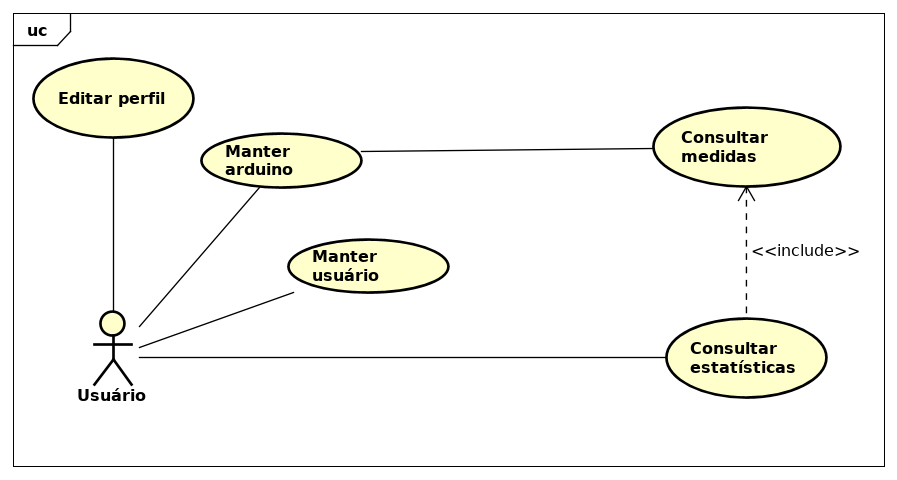
\includegraphics[scale=0.6]{diagrams/caso_de_uso.png}
    \hfill
\end{figure}

Os atores do sistema foram definidos como os sensores, que podem realizar o cadastro de capturas e o usuário, que fará o cadastro de usuários e estações meteorológicas.
Seguem abaixo as especificações dos casos de uso.

\begin{table}[H]
    \ABNTEXfontereduzida
    \caption{Especificações do caso de uso capturar dados meteorológicos}
    \label{my-label}
    \begin{tabular}{{l}|p{11.5cm}}

    \hline

    \multicolumn{2}{c}{\textbf{Capturar dados meteorológicos}} \\

    \hline
    Descrição & Captura os dados meteorológicos através de sensores conectados ao microcontrolador arduino e os envia através de requisição HTTP para a API \\

    \hline

    Atores & Sistema \\

    \hline

    \multirow{2}{*}{Pré-condições} & Credenciais de acesso a API \\
    & API em correto funcionamento \\

    \hline

    \end{tabular}
\end{table}

\begin{table}[H]
    \ABNTEXfontereduzida
    \caption{Especificações do caso de uso armazenar dados meteorológicos}
    \label{my-label}
    \begin{tabular}{{l}|p{9.0cm}}

    \hline

    \multicolumn{2}{c}{\textbf{Armazenar dados meteorológicos}} \\

    \hline
    Descrição & Após receber os dados captados pelo arduino, a api os valida e então, os armazena em banco de dados \\

    \hline

    Atores & Sistema \\

    \hline

    \multirow{2}{*}{Pré-condições} & Banco de dados em correto funcionamento  \\
    & Recebimento de dados através das rotas da API \\

    \hline

    \multirow{2}{*}{Exceções e fluxos alternativos} & Em caso de dados inválidos, a API os descarta \\

    & Em caso de perca de conexão com banco de dados, a API os armazena em memória \\

    \hline

    \end{tabular}
\end{table}

\begin{table}[H]
    \ABNTEXfontereduzida
    \caption{Especificações do caso de uso realizar consultas com filtros}
    \label{my-label}
    \begin{tabular}{{l}|p{9.0cm}}

    \hline

    \multicolumn{2}{c}{\textbf{Realizar consultas com filtros}} \\

    \hline
    Descrição & Recebe do usuário os filtros para seleção das informações, então, realiza uma análise estatística dos dados requeridos e os exibe para o usuário utilizando gráficos. \\

    \hline

    Atores & Usuário \\

    \hline

    \multirow{3}{*}{Pré-condições} & Credenciais de acesso ao banco de dados para realizar as consultas  \\
    & Banco de dados em correto funcionamento \\
    & Filtros corretos passados pelo usuário \\

    \hline

    \multirow{2}{*}{Exceções e fluxos alternativos} & Caso ele não encontre dados na seleção, exibe uma mensagem de não encontrado  \\

    & Em caso de perca de conexão com banco de dados, exibe uma tela de erro ao usuário \\

    \hline

    \end{tabular}
\end{table}

\begin{table}[H]
    \ABNTEXfontereduzida
    \caption{Especificações do caso de uso realizar análise estatística dos dados}
    \label{my-label}
    \begin{tabular}{{l}|p{9.0cm}}

    \hline

    \multicolumn{2}{c}{\textbf{Realizar análise estatística dos dados}} \\

    \hline
    Descrição & Realiza calculo estatístico de informações, retornando informações relevantes como média, moda e desvio padrão. \\

    \hline

    Atores & Usuário \\

    \hline

    \multirow{2}{*}{Pré-condições} & Credenciais de acesso ao banco de dados  \\
    & Banco de dados em correto funcionamento \\

    \hline

    \multirow{2}{*}{Exceções e fluxos alternativos} & Caso não existam dados para serem analisados, joga uma exceção de argumentos inválidos  \\

    \end{tabular}
\end{table}

\section{Requisitos não funcionais}

Os requisitos não funcionais do sistema complementam os requisitos funcionais, como melhorias para as especificações.

\subsection{Segurança}

O projeto precisa trabalhar de forma segura, então, esse requisito pede para que a API possua autenticação das aplicações clientes e que também, a aplicação web possua autenticação, para o usuário visualizar as informações e realizar consultas, ele precisa estar autenticado.

\subsection{Disponibilidade}

Para garantir uma melhor análise e fidelidade dos dados, o sistema precisa funcionar durante 24 horas por dia e 7 dias por semana, para isso, redundâncias precisam ser trabalhadas.

\subsection{Performance}

Outro requisito não funcional do sistema é a performance, as informações precisam ser processadas de forma rápida, problemas como lentidão no processamento podem acabar travando a entrada de dados no sistema.

% ----------------------------------------------------------
% c/Análise dos dados capturados
% ----------------------------------------------------------
\chapter{Análise dos dados capturados}
\addcontentsline{toc}{chapter}{Análise dos dados capturados}

As informações que foram capturadas pelo microcontrolador, ao serem requisitadas pelo usuário, são disponibilizadas através de uma interface gráfica, utilizando análise de estatística e gráficos.

\section{Filtros}

Os filtros utilizados pelo usuário, são a estação meteorológica que ele deseja visualizar, a data inicial e a data final para busca dos dados e o intervalo para calculo das médias.

\subsection{Tratamento de dados}

Os dados foram exibidos da mesma forma que foram capturados, com exceção das informações de intensidade de luz, que foi invertida para melhor exibição no gráfico, e pela medida de nível de chuva, que além de invertida, foi transformada em porcentagem.

\section{Resultados}

\subsection{Médias}

A média aplicada em cima dos dados, é separada por um intervalo de tempo, como exemplo, caso o usuário informe que o intervalo requisitado é de uma hora, os dados são agrupados por cada hora e então, uma média é aplicada nesses dados, exibindo as médias em intervalos de horas no gráfico.

\subsection{Mínimas e Máximas}

É exibida também uma lista com as mínimas e máximas daquela estação meteorológica no intervalo de tempo informado.

% ----------------------------------------------------------
% c/Diagrama de classes
% ----------------------------------------------------------
\chapter{Diagrama de classes}
\addcontentsline{toc}{chapter}{Diagrama de classes}

Como podemos verificar no diagrama descrito na figura \ref{figure_diagrama_classe} as entidades do sistema consistem na medida, que é a informação que foi capturada pelo arduino, as entidades arduino e usuário também estão presentes, todas extendem da Model do Mongoose.

\begin{figure}[H]
    \label{figure_diagrama_classe}
    \centering
    \caption{Diagrama de classes}
    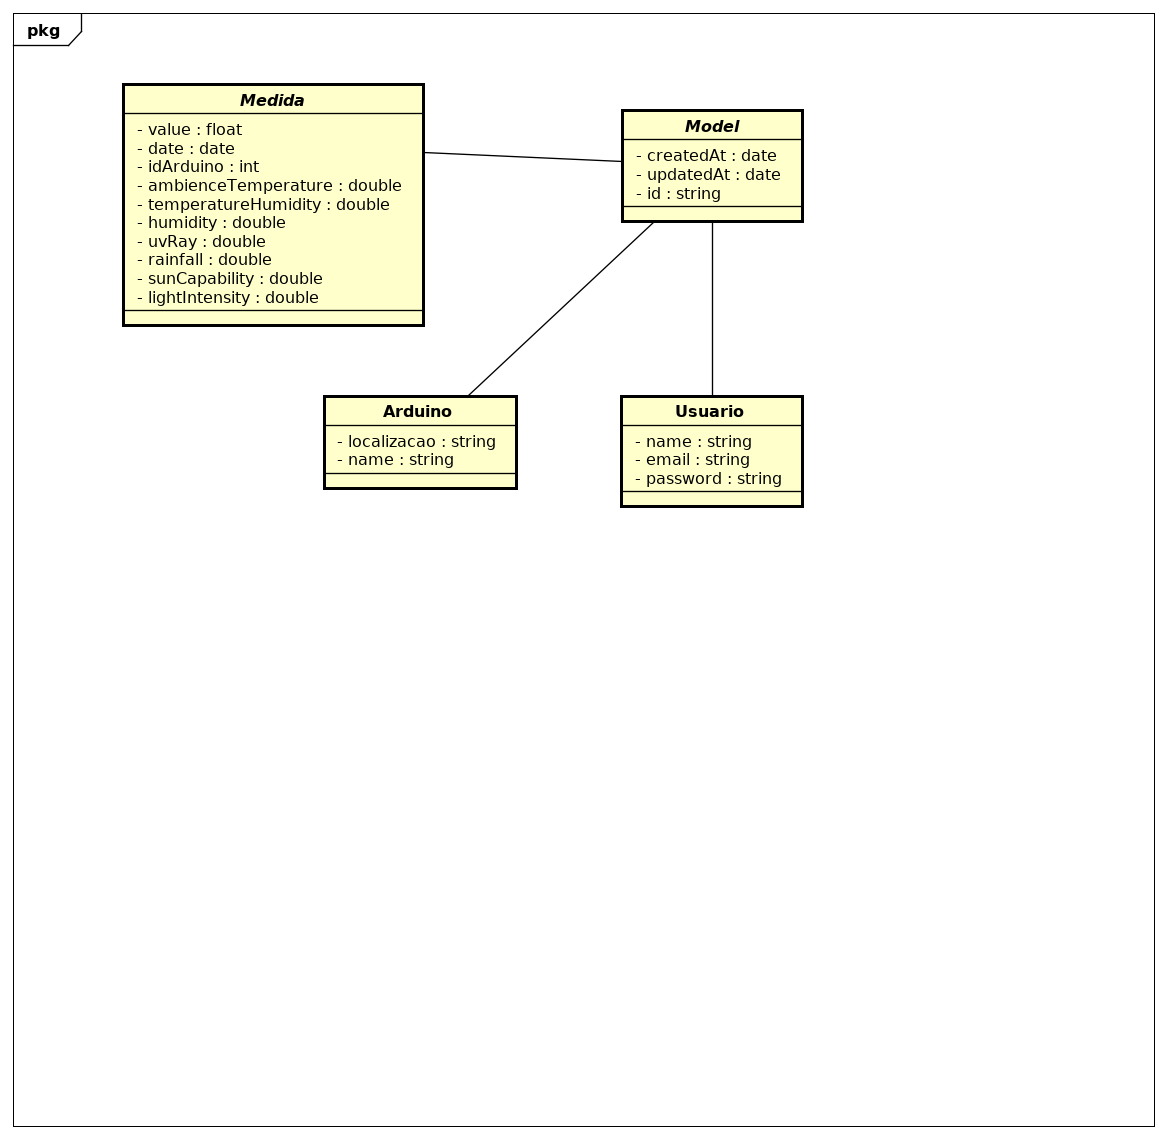
\includegraphics[scale=0.5]{diagrams/classe.png}
    \hfill
\end{figure}

% ----------------------------------------------------------
% c/Diagrama de sequência
% ----------------------------------------------------------
\chapter{Diagrama de sequência}
\addcontentsline{toc}{chapter}{Diagrama de sequência}

Apresentação do diagrama de sequencia do projeto.

\begin{figure}[H]
    \label{figure_diagrama_sequencia}
    \centering
    \caption{Diagrama de sequência}
    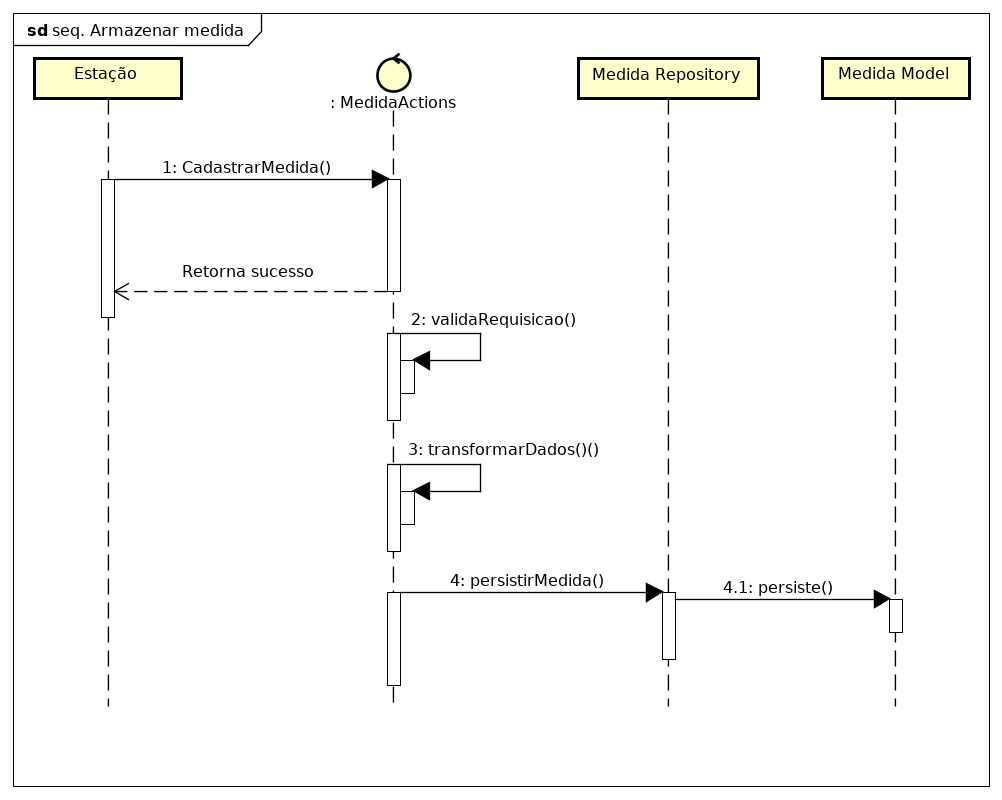
\includegraphics[scale=0.40]{diagrams/sequencia.png}
    \hfill
\end{figure}

Como descrito no diagrama de sequência representado na figura \ref{figure_diagrama_sequencia} a aplicação é composta por 3 principais camadas.

\section{Controlador}

Na camada de controle, os dados são recebidos e passam por uma básica validação através, porém não sofrem a interferência das regras de negócio.

Nessa camada, os dados são recebidos e retornados ao cliente, é uma interface de acesso a aplicação, geralmente, essa camada recebe objetos de requisições HTTP.

\section{Serviço}

Na camada de serviço as ações são os casos de uso, o caso de uso responsável por aquela ação trabalha, inserindo os dados através do repositório no banco de dados, e então, retorna as informações.

\section{Repositório}

Dentro da camada de repositório, são recebidos dados que, através de uma camada de infraestrutura são persistidos, retornando então, uma entidade.

% ----------------------------------------------------------
% c/Diagrama de estado
% ----------------------------------------------------------
\chapter{Diagrama de estado}
\addcontentsline{toc}{chapter}{Diagrama de estado}

Apresentação dos estados de uma entidade de medida que foi capturada ao longo da interação com o sistema.

\begin{figure}[H]
    \label{figure_diagrama_estado}
    \centering
    \caption{Diagrama de estado}
    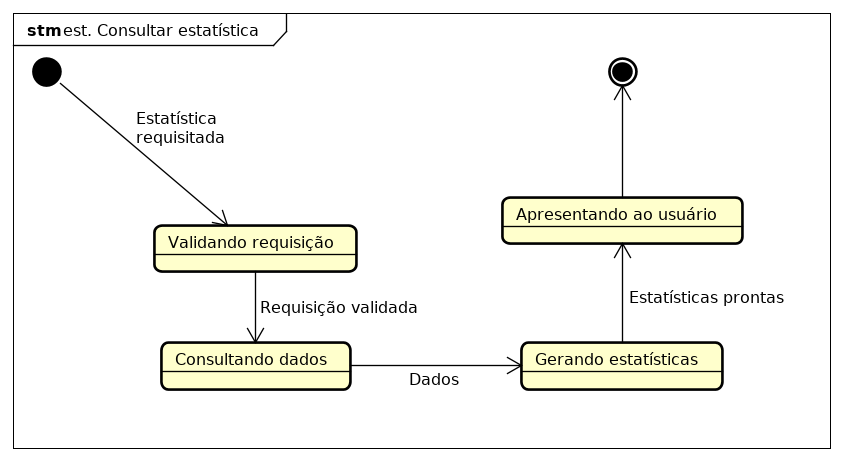
\includegraphics[scale=0.6]{diagrams/estado.png}
    \hfill
\end{figure}

Conforme descrito na figura \ref{figure_diagrama_estado} os estados durante o armazenamento de uma de uma medida são:

\section{Validando requisição}

A autenticação do arduino na API foi feita e a requisição HTTP para o armazenamento de uma medida foi feita até a API.
Nesse estado, a requisição está passando por uma validação básica, verificando os tipos e formato dos dados.

\section{Armazenando em banco de dados}

A medida é valida e está sendo armazenada no banco de dados, após, ela é retornada a camada de serviço.

% ----------------------------------------------------------
% c/Diagrama de implementação
% ----------------------------------------------------------
\chapter{Diagrama de implementação}
\addcontentsline{toc}{chapter}{Diagrama de implementação}

A seguir o diagrama de implementação do sistema, que descreve a forma como os componentes de hardware e software interagem entre si.

\begin{figure}[H]
    \label{figure_diagrama_implementacao}
    \centering
    \caption{Diagrama de implementação}
    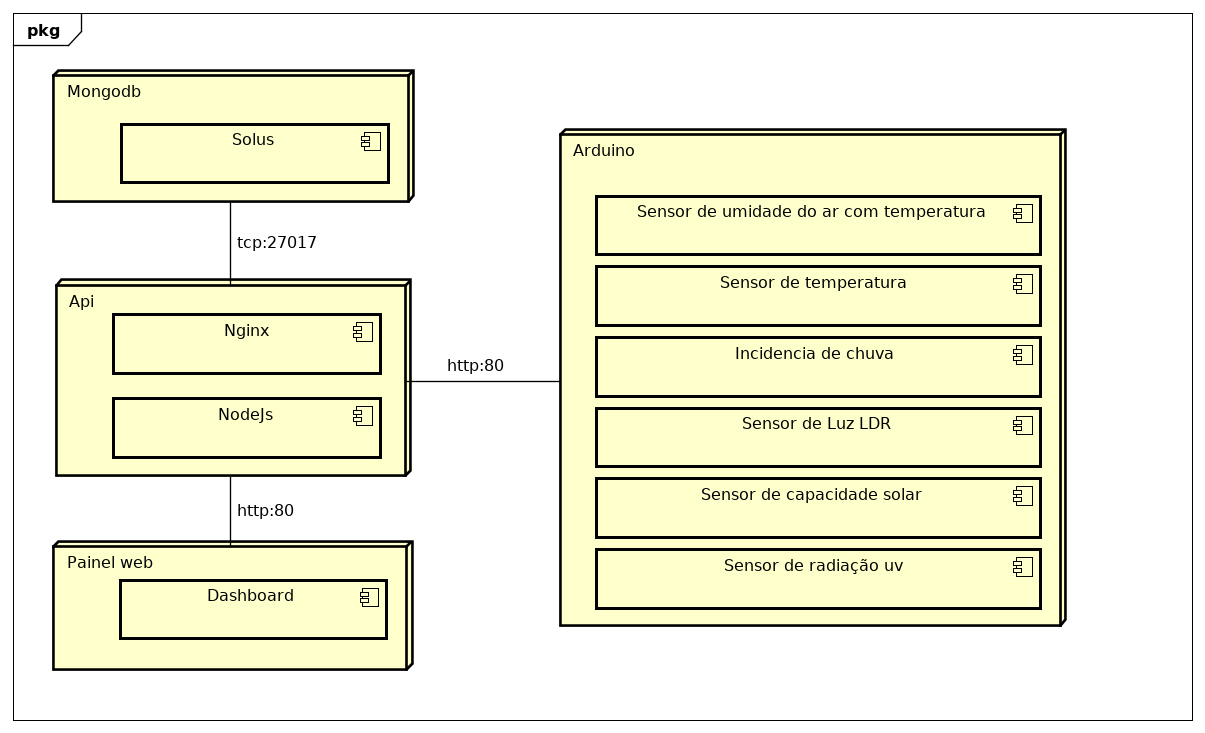
\includegraphics[scale=0.6]{diagrams/implementacao.png}
    \hfill
\end{figure}

\section{Sensores}

Os sensores do arduino, são ligados através da protoboard até o arduino, onde a captação é feita e as informações são tratadas, os dados são montados dentro de uma string JSON, que é enviada para o nodeMCU.

Não foi utilizada a biblioteca para a montagem da string JSON por conta da memória limitada do controlador.

\section{NodeMCU}

Na placa de WiFi NodeMCU, as informações são recebidas através da porta serial e o json recebido é enviado para a api.

% ----------------------------------------------------------
% c/Descrição e documentação da API
% ----------------------------------------------------------
\chapter{Descrição e documentação da API}
\addcontentsline{toc}{chapter}{Descrição e documentação da API}

Podemos conferir abaixo a documentação das rotas da API.

\begin{table}[H]
    \centering
    \caption{Descrição das rotas da API}
    \label{table_api_routes}
    \begin{tabular}{|l|l|l|}
    \hline
    \textbf{Método}  & \textbf{Rota}        & \textbf{Descrição}                           \\ \hline
    GET              & /arduino             & Lista os arduinos                            \\ \hline
    GET              & /arduino/:id         & Retorna os dados de um arduino               \\ \hline
    POST             & /arduino             & Cadastra um novo arduino                     \\ \hline
    POST, PATCH, PUT & /arduino/:id         & Atualiza os dados de um arduino              \\ \hline
    DELETE           & /arduino/:id         & Deleta um arduino e suas medidas capturadas  \\ \hline
    GET              & /user                & Lista os usuários                            \\ \hline
    GET              & /user/:id            & Retorna os dados de um usuário               \\ \hline
    POST             & /user                & Cadastra um novo usuário                     \\ \hline
    POST, PATCH, PUT & /user/:id            & Atualiza os dados de um usuário              \\ \hline
    DELETE           & /user/:id            & Deleta um usuário                            \\ \hline
    POST             & /user/login          & Recebe as credenciais e retorna o token      \\ \hline
    POST             & /measure             & Cadastra uma medida capturada                \\ \hline
    GET              & /statistic/:id       & Retorna as estatísticas de dados do arduino  \\ \hline
    \end{tabular}
\end{table}

\section{Métodos HTTP utilizados}

Como podemos visualizar na tabela \ref{table_api_routes}, o método POST fica designado a criar um recurso quando a requisição for enviada para uma rota sem a identificação. O método POST também é utilizado para atualizar um recurso quando a requisição for enviada para um recurso identificado. Para a atualização de um recurso também pode ser utilizado o método PATCH.
Para a consulta de recursos é utilizado o método GET, o método DELETE é utilizado para excluir um recurso.

\section{Autenticação}

A autenticação foi feita utilizando Json Web Token, onde, uma vez que o usuário tenha feito o login na API, as informações do usuário e seu token de acesso são retornados.

O token é passado para as rotas através dos cabeçalhos da requisição, onde a autenticação se faz necessária, o token enviado é validado, e caso seja invalido, o acesso ao usuário é negado.

% ----------------------------------------------------------
% Finaliza a parte no bookmark do PDF
% para que se inicie o bookmark na raiz
% e adiciona espaço de parte no Sumário
% ----------------------------------------------------------
\phantompart

% ----------------------------------------------------------
% c/Conclusão
% ----------------------------------------------------------
\chapter{Conclusão}
% ---

Conclusão
